\chapter{साम्य स्थिरांक और साम्य का विस्थापन}\label{ch:b2:equilibrium-shifts}

अमोनिया संयंत्र अपना परिवर्तक लगभग \qty{450}{\celsius} और
\qty{200}{bar} पर चलाता है। कमरे के ताप पर \ce{N2 + 3H2 <=>
2NH3} का साम्य अमोनिया की ओर इतना अधिक होता है कि तत्वों का मिश्रण
सिद्धांततः लगभग पूरा रूपांतरित हो सकता है; फिर भी इंजीनियर उसे गर्म करते हैं, जिससे
साम्य पीछे खिसकता है, और फिर उसे दो सौ वायुमंडल तक संपीडित करते हैं, जिसमें
बहुत ऊर्जा लगती है। इसके कारण इस बात के बीच का समझौता हैं कि अभिक्रिया कितनी
आगे जा सकती है और कितनी तेज़ी से चलती है। यह अध्याय पिछले अध्यायों की
\omterm{def:b2:reaction-free-energy:gibbs-energy}{गिब्स ऊर्जा} को प्रथम वर्ष के खंड के साम्य स्थिरांक में बदलता है, दिखाता है कि
वह स्थिरांक ताप के साथ कैसे बदलता है, गिनता है कि प्रयोगकर्ता कितनी परिस्थितियाँ
स्वतंत्र रूप से चुन सकता है, और पूर्वानुमान करता है कि ताप, दाब या संघटन
बदलने पर साम्य किस दिशा में खिसकता है।

\begin{recall}
\Cref{ch:b2:reaction-free-energy}: विकास निकष $\Delta_r G\,\dd\xi
\leq 0$ और गिब्स--हेल्महोल्ट्ज़ संबंध;
\cref{ch:b2:chemical-potential}: $\Delta_r G = \Delta_r G^\circ + RT\ln Q$।
प्रथम वर्ष का खंड: भागफल $Q = \prod_i a_i^{\nu_i}$, मानक
साम्य स्थिरांक $K^\circ$ साम्य पर $Q$ के मान के रूप में, द्रव्य-अनुपाती क्रिया
का नियम और नियम ``$Q < K^\circ$: अग्र'', ये सब वहाँ नियमों के रूप में
कहे गए थे; प्रगति सारणियाँ; एक या दो अभिक्रियाओं की अंतिम अवस्थाएँ। उसने यह
वचन भी दिया था कि अमोनिया और सल्फ़र ट्राइऑक्साइड के लिए ताप और दाब के चुनाव
की व्याख्या यहाँ की जाएगी।
\end{recall}

\begin{omfigure}
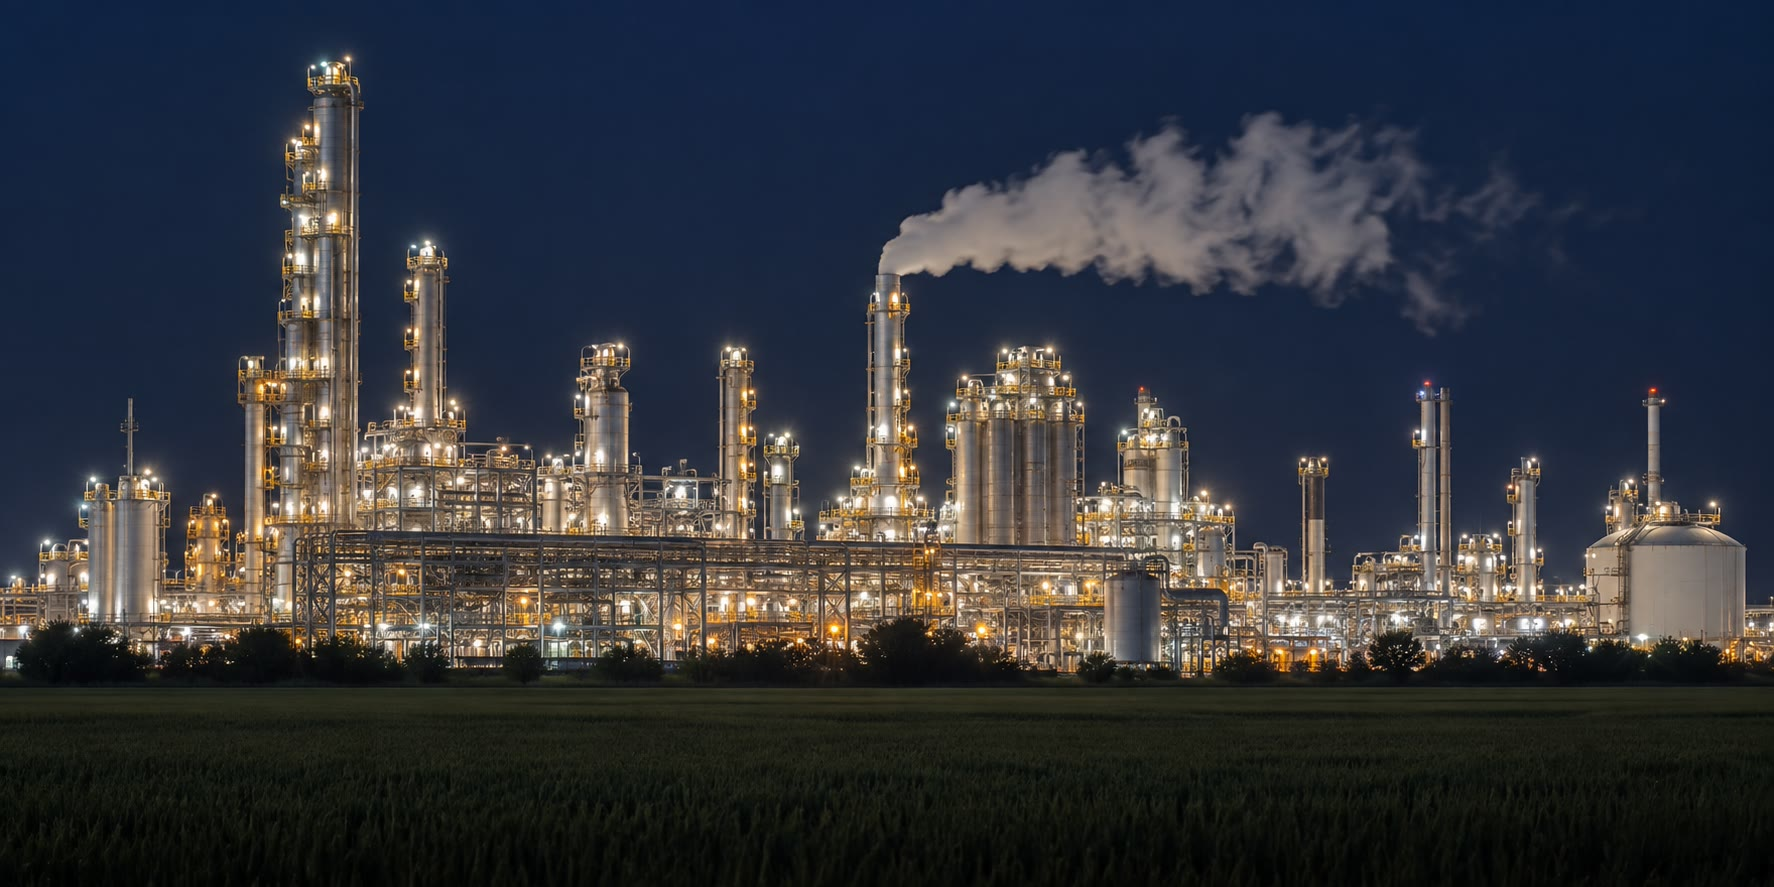
\includegraphics[width=0.7\linewidth]{images/book3/ai/b2-04-ammonia-plant.jpg}

{\small रात में एक अमोनिया संयंत्र। इसके परिवर्तक में नाइट्रोजन और हाइड्रोजन
कुछ सौ डिग्री और कुछ सौ \unit{bar} पर लोहे के उत्प्रेरक के ऊपर से गुज़रती हैं;
इन परिस्थितियों का चुनाव सप्ताहांत समस्या का विषय है।}
\end{omfigure}

\section{गिब्स ऊर्जा से साम्य स्थिरांक}

\begin{theorem}[मानक साम्य स्थिरांक]\label{thm:b2:equilibrium-shifts:k-from-g}
साम्य पर $\Delta_r G = 0$, और अभिक्रिया भागफल यह मान लेता है:
\[
  K^\circ(T) = \exp\!\left(-\frac{\Delta_r G^\circ(T)}{RT}\right), \qquad
  \Delta_r G^\circ(T) = -RT\ln K^\circ(T) .
\]
यह केवल ताप पर निर्भर करता है।
\end{theorem}

\begin{proof}
विकास निकष $\Delta_r G = 0$ को साम्य की शर्त बनाता है।
$\Delta_r G = \Delta_r G^\circ + RT\ln Q$
(\cref{prop:b2:chemical-potential:delta-g-q}) के साथ, साम्य का अर्थ है $\ln Q_{\text{साम्य}}
= -\Delta_r G^\circ/(RT)$, जो केवल $T$ का फलन है क्योंकि $\Delta_r G^\circ$ भी है।
\end{proof}

\begin{corollary}[प्रथम वर्ष के खंड के नियम]\label{cor:b2:equilibrium-shifts:mass-action}
$\Delta_r G = RT\ln(Q/K^\circ)$। अतः $Q < K^\circ$ वाला निकाय अग्र दिशा में
विकसित होता है, $Q > K^\circ$ वाला पश्च दिशा में, और $Q = K^\circ$ वाला
साम्य में है (द्रव्य-अनुपाती क्रिया का नियम)।
\end{corollary}

\begin{proof}
$\Delta_r G^\circ = -RT\ln K^\circ$ को $\Delta_r G = \Delta_r G^\circ
+ RT\ln Q$ में रखिए; $\Delta_r G$ का चिह्न $\ln(Q/K^\circ)$ का चिह्न है, और
विकास निकष $\Delta_r G\,\dd\xi \leq 0$ माँगता है।
\end{proof}

\begin{example}[\qty{298}{K} पर तीन स्थिरांक]\label{ex:b2:equilibrium-shifts:constants}
अमोनिया संश्लेषण, $\Delta_r G^\circ = \qty{-32.8}{kJ/mol}$: $K^\circ =
\exp(32\,800/(8.314 \times 298.15)) = \num{5.6e5}$ (अधिक अंकों वाली सारणियाँ
\num{5.4e5} देती हैं)। \ce{N2O4} का वियोजन, $\Delta_r G^\circ =
\qty{+4.7}{kJ/mol}$: $K^\circ = 0.15$। चूना पत्थर का विघटन,
$\Delta_r G^\circ = \qty{+130.4}{kJ/mol}$: $K^\circ = \num{1.5e-23}$, और
कमरे के ताप पर चूना पत्थर के ऊपर कार्बन डाइऑक्साइड का साम्य दाब
$\num{1.5e-23}$~\unit{bar} है, अर्थात् कुछ भी नहीं। \qty{298}{K} पर $\Delta_r G^\circ$ में
\qty{5.7}{kJ/mol} का परिवर्तन $K^\circ$ को दस से गुणा या भाग कर देता है।
% ledger: dfh:NH3_g, s0:NH3_g, janafG:NH3.298.15 (computed in figdata/bachelor-2/thermo-data.py and vant-hoff.py)
\end{example}

पूरे निकाय की \omterm{def:b2:reaction-free-energy:gibbs-energy}{गिब्स ऊर्जा} यही बात एक भू-दृश्य के रूप में दिखाती है:
वह साम्य प्रगति पर न्यूनतम होती है, जहाँ उसकी प्रवणता, $\Delta_r G$,
शून्य है।

\begin{omfigure}
\begin{tikzpicture}
\begin{axis}[
  width=0.7\linewidth, height=5.6cm, xmin=0, xmax=1, ymin=-2.2, ymax=5.2,
  axis x line=bottom, axis y line=left, xlabel={प्रगति $\xi$ (mol)},
  ylabel={$G(\xi) - G(0)$ (\unit{kJ})},
  tick label style={font=\small}, label style={font=\small}, clip=false]
\addplot[omDef, very thick] table[x=xi, y=G] {figdata/out/bachelor-2-gibbs-extent.dat};
\draw[dotted] (axis cs:0.189,-2.2) -- (axis cs:0.189,-0.949);
\fill[omThm] (axis cs:0.189,-0.949) circle (1.6pt);
\node[omThm, anchor=west, font=\small] at (axis cs:0.21,-1.75) {साम्य, $\xi = 0.189$};
\draw[dashed, gray] (axis cs:0,0) -- (axis cs:1,4.728);
\node[gray, font=\scriptsize, anchor=south east] at (axis cs:1,4.75) {$\xi\,\Delta_r G^\circ$};
\end{axis}
\end{tikzpicture}

{\small \qty{298}{K} और \qty{1}{bar} पर आदर्श गैसों के एक बंद निकाय की \omterm{def:b2:reaction-free-energy:gibbs-energy}{गिब्स ऊर्जा},
\ce{N2O4} के \qty{1}{mol} से आरंभ करके,
\ce{N2O4 <=> 2NO2} की प्रगति के सापेक्ष। यद्यपि $\Delta_r G^\circ > 0$ (खंडित रेखा, शुद्ध
स्पीशीज़), दोनों गैसों का मिश्रण $G$ को घटाता है, और न्यूनतम $\xi =
0.189$ पर है, जहाँ $Q = K^\circ = 0.15$। इसके बाईं ओर प्रवणता $\Delta_r G =
\partial G/\partial\xi$ ऋणात्मक है, दाईं ओर धनात्मक।}
% ledger: dfh:N2O4_g, s0:N2O4_g, dfh:NO2_g, s0:NO2_g (computed in figdata/bachelor-2/gibbs-extent.py)
\end{omfigure}

\section{ताप: वांट हॉफ़ समीकरण}

\begin{theorem}[वांट हॉफ़ समीकरण]\label{thm:b2:equilibrium-shifts:vant-hoff}
\[
  \frac{\dd\ln K^\circ}{\dd T} = \frac{\Delta_r H^\circ(T)}{RT^2}
\]
(\emph{वांट हॉफ़ समीकरण}\index{वांट हॉफ़ समीकरण}): \omterm{def:b2:reaction-enthalpy:exothermic}{ऊष्माशोषी} अभिक्रिया का
साम्य स्थिरांक ताप के साथ बढ़ता है, \omterm{def:b2:reaction-enthalpy:exothermic}{ऊष्माक्षेपी} अभिक्रिया का
घटता है।
\end{theorem}

\begin{proof}
$\ln K^\circ = -\Delta_r G^\circ/(RT)$ लिखिए और
\cref{prop:b2:reaction-free-energy:gibbs-helmholtz} के गिब्स--हेल्महोल्ट्ज़ संबंध का उपयोग कीजिए,
\[
  \frac{\dd}{\dd T}\left(\frac{\Delta_r G^\circ}{T}\right) =
  -\frac{\Delta_r H^\circ}{T^2} ;
\]
$-R$ से भाग दीजिए।
\end{proof}

\begin{proposition}[समाकलित रूप]\label{prop:b2:equilibrium-shifts:integrated}
यदि $\Delta_r H^\circ$, $T_1$ और $T_2$ के बीच स्थिर है (\omterm{def:b2:reaction-free-energy:ellingham-approximation}{एलिंगम
सन्निकटन}),
\[
  \ln\frac{K^\circ(T_2)}{K^\circ(T_1)} = -\frac{\Delta_r H^\circ}{R}\left(
  \frac{1}{T_2} - \frac{1}{T_1}\right),
\]
और $\ln K^\circ$ एक सरल रेखा है जिसकी प्रवणता $-\Delta_r H^\circ/R$ है,
$1/T$ के सापेक्ष।
\end{proposition}

\begin{proof}
$\dd\ln K^\circ = (\Delta_r H^\circ/R)\,\dd T/T^2$ का समाकलन कीजिए, यह ध्यान रखते हुए कि
$\dd T/T^2 = -\dd(1/T)$।
\end{proof}

\begin{omfigure}
\begin{tikzpicture}
\begin{axis}[
  width=0.72\linewidth, height=5.8cm, xmin=0.9, xmax=3.5, ymin=-19, ymax=15,
  axis x line=bottom, axis y line=left, xlabel={$1000/T$ (\unit{1/K})},
  ylabel={$\ln K^\circ$}, tick label style={font=\small},
  label style={font=\small}, clip=false]
\addplot[omThm, dashed, thick] table[x=invT, y=lnK] {figdata/out/bachelor-2-vant-hoff-a-line.dat};
\addplot[omDef, only marks, mark=*, mark size=1.8pt] table[x=invT, y=lnK] {figdata/out/bachelor-2-vant-hoff-a.dat};
\node[omDef, font=\scriptsize, anchor=west] at (axis cs:3.36,13.2) {\qty{298}{K}};
\node[omDef, font=\scriptsize, anchor=north west] at (axis cs:1.03,-15.3) {\qty{1000}{K}};
\node[omThm, font=\small, anchor=south east, align=right] at (axis cs:2.4,8) {प्रवणता $-\Delta_r H^\circ(298)/R$\\ $= +11\,050$ K};
\end{axis}
\end{tikzpicture}

{\small सारणियों से \ce{N2 + 3H2 <=> 2NH3} का स्थिरांक (बिंदु, 298 से
\qty{1000}{K}) और \qty{298}{K} वाले $\Delta_r H^\circ$ से खींची गई वांट हॉफ़
रेखा (खंडित)। अभिक्रिया \omterm{def:b2:reaction-enthalpy:exothermic}{ऊष्माक्षेपी} है: $K^\circ$
\num{5e5} से \num{3e-7} तक गिरता है। उच्च ताप पर बिंदु रेखा से नीचे आ जाते हैं:
$\Delta_r H^\circ$ अधिक ऋणात्मक होता जाता है जैसे-जैसे $T$ बढ़ता है
(\cref{ex:b2:reaction-enthalpy:kirchhoff})।}
% ledger: janafG:NH3.298.15, janafG:NH3.400, janafG:NH3.500, janafG:NH3.600, janafG:NH3.700, janafG:NH3.800, janafG:NH3.900, janafG:NH3.1000, dfh:NH3_g (computed in figdata/bachelor-2/vant-hoff.py)
\end{omfigure}

\begin{method}[किसी दूसरे ताप पर साम्य स्थिरांक]\label{met:b2:equilibrium-shifts:k-at-t}
\begin{enumerate}
  \item \qty{298}{K} की सारणियों से $\Delta_r H^\circ$, $\Delta_r
        S^\circ$, और $K^\circ(298)$ परिकलित कीजिए।
  \item या तो समाकलित \omterm{thm:b2:equilibrium-shifts:vant-hoff}{वांट हॉफ़ समीकरण} का उपयोग कीजिए, या
        $\Delta_r G^\circ(T) = \Delta_r H^\circ - T\Delta_r S^\circ$ और फिर
        $K^\circ(T)$ परिकलित कीजिए: दोनों एक ही सन्निकटन हैं।
  \item चौड़े अंतराल या बड़े $\Delta_r C_p^\circ$ के लिए सारणीबद्ध
        $\Delta_f G^\circ(T)$ को प्राथमिकता दीजिए; \qty{298}{K} पर \qty{5.7}{kJ/mol}
        (या \qty{700}{K} पर \qty{13}{kJ/mol}) की त्रुटि $K^\circ$ में दस का गुणक है।
\end{enumerate}
\end{method}

\begin{history}[याकोबस हेनरिकस वांट हॉफ़]
\begin{minipage}[t]{0.2\linewidth}\vspace{0pt}
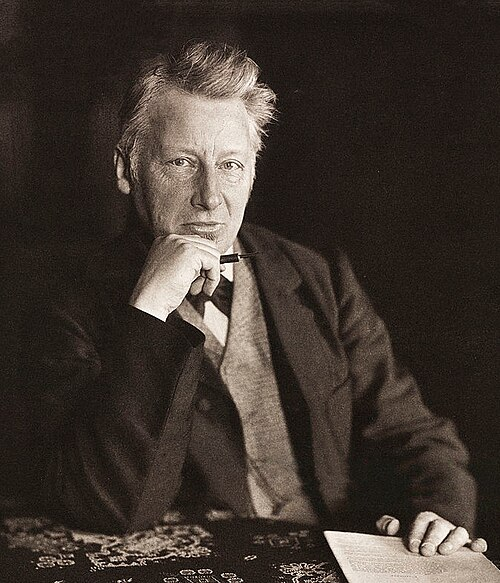
\includegraphics[width=\linewidth]{images/book3/vanthoff.jpg}
\end{minipage}\hfill
\begin{minipage}[t]{0.76\linewidth}\vspace{0pt}
याकोबस हेनरिकस वांट हॉफ़ (1852--1911) ने 1884 में अपनी
\emph{रासायनिक गतिकी के अध्ययन} में ताप और
साम्य स्थिरांक के बीच वह संबंध दिया जो उनके नाम से जाना जाता है, और अगले वर्ष
\cref{ch:b2:chemical-potential} का \omterm{def:b2:chemical-potential:osmotic-pressure}{परासरण दाब} नियम; दस वर्ष पहले उन्होंने
चतुष्फलकीय कार्बन परमाणु प्रस्तावित किया था। उन्हें 1901 में रसायन का पहला
नोबेल पुरस्कार मिला। (छायाचित्र: न॰ पर्शाइड, 1904; सार्वजनिक अधिकार-क्षेत्र,
विकिमीडिया कॉमन्स।)
\end{minipage}
\end{history}

\section{स्वातंत्र्य कोटि}

साम्य अवस्था के पूर्णतः निर्धारित होने से पहले प्रयोगकर्ता कितनी गहन राशियाँ
स्वतंत्र रूप से नियत कर सकता है?

\begin{definition}[स्वातंत्र्य कोटि]\label{def:b2:equilibrium-shifts:variance}
साम्य में किसी निकाय के \emph{स्वतंत्र गहन प्राचल}\index{स्वतंत्र गहन प्राचल}
गहन राशियों का ऐसा समुच्चय हैं
(ताप, दाब, हर प्रावस्था में मोल अंश) जिन्हें
स्वतंत्र रूप से चुना जा सकता है और जो, एक बार चुन लिए जाने पर, शेष सबको नियत कर देते हैं। उनकी संख्या
निकाय की \emph{स्वातंत्र्य कोटि}\index{स्वातंत्र्य कोटि} $v$ है।
\end{definition}

\begin{theorem}[प्रावस्था नियम]\label{thm:b2:equilibrium-shifts:phase-rule}
$n$ स्पीशीज़ के ऐसे निकाय के लिए, जो $\varphi$ प्रावस्थाओं में वितरित हैं और $r$
स्वतंत्र साम्य अभिक्रियाओं और तैयारी द्वारा नियत, गहन राशियों के बीच $s$
अतिरिक्त संबंधों (रससमीकरणमितीय फ़ीड,
विद्युत-उदासीनता) से जुड़ी हैं,
\[
  v = c + 2 - \varphi, \qquad c = n - r - s .
\]
\end{theorem}

\begin{proof}
गहन चर: $T$, $p$, और हर प्रावस्था में
$n$ स्पीशीज़ के मोल अंश, जिनका योग 1 है, अतः प्रति प्रावस्था $n - 1$ स्वतंत्र: कुल $2 +
\varphi(n - 1)$। संबंध: हर स्पीशीज़ प्रावस्थाओं के बीच साम्य में है,
प्रति स्पीशीज़ \omterm{def:b2:chemical-potential:chemical-potential}{रासायनिक विभवों} की $\varphi - 1$ समताएँ, कुल $n(\varphi -
1)$; हर अभिक्रिया $Q = K^\circ(T)$ देती है, $r$ संबंध; और $s$
अतिरिक्त संबंध। घटाइए: $v = 2 + \varphi(n - 1) - n(\varphi - 1) - r -
s = n - r - s + 2 - \varphi$। (किसी प्रावस्था में अनुपस्थित स्पीशीज़ एक
चर और एक संबंध साथ-साथ हटा देती है।)
\end{proof}

\begin{method}[स्वातंत्र्य कोटि का परिकलन]\label{met:b2:equilibrium-shifts:variance}
\begin{enumerate}
  \item स्पीशीज़ को उनकी प्रावस्था सहित सूचीबद्ध कीजिए, और $n$ तथा $\varphi$ गिनिए
        (हर शुद्ध ठोस एक प्रावस्था है; सभी गैसें मिलकर एक प्रावस्था बनाती हैं)।
  \item उनके बीच स्वतंत्र अभिक्रियाएँ $r$ गिनिए।
  \item अतिरिक्त संबंध $s$ गिनिए: रससमीकरणमितीय अनुपात में मात्राएँ
        (केवल यदि संबंध एक ही प्रावस्था की राशियों के बीच हो),
        आयनिक विलयन की विद्युत-उदासीनता।
  \item $v = n - r - s + 2 - \varphi$।
\end{enumerate}
\end{method}

\begin{example}[तीन स्वातंत्र्य कोटियाँ]\label{ex:b2:equilibrium-shifts:variances}
बंद पात्र में चूना पत्थर, \ce{CaCO3(s) <=> CaO(s) + CO2(g)}: $n = 3$, $r =
1$, $\varphi = 3$ (दो ठोस, एक गैस): $v = 1$। $T$ चुनिए, और कार्बन डाइऑक्साइड
का दाब नियत हो जाता है: $p = K^\circ(T)\,p^\circ$। साम्य पर
\ce{N2}, \ce{H2} और \ce{NH3} का गैस मिश्रण: $n = 3$, $r = 1$, $\varphi = 1$, $v
= 3$ ($T$, $p$ और संघटन का एक चर); केवल अमोनिया से, या
रससमीकरणमितीय फ़ीड से बनाने पर \ce{N2} और \ce{H2} 1 : 3 के अनुपात में होते हैं, $s = 1$ और
$v = 2$: दिए गए $T$ और $p$ पर संघटन नियत है, जिसका उपयोग सप्ताहांत समस्या
करती है।
\end{example}

\section{साम्य का विस्थापन}

\begin{definition}[साम्य का विस्थापन]\label{def:b2:equilibrium-shifts:shift}
जब साम्य में किसी निकाय को विक्षुब्ध किया जाता है (ताप, दाब, या किसी मात्रा
का परिवर्तन), तो वह सामान्यतः साम्य में नहीं रहता और एक नए साम्य की ओर
विकसित होता है। \emph{साम्य का विस्थापन}\index{साम्य का विस्थापन}
अग्र है यदि अभिक्रिया आगे बढ़ती है ($\dd\xi > 0$), अन्यथा
पश्च।
\end{definition}

\begin{method}[विस्थापन का पूर्वानुमान]\label{met:b2:equilibrium-shifts:predict-shift}
विक्षोभ के ठीक बाद $Q$ और $K^\circ$ परिकलित कीजिए (या उनके परिवर्तन के चिह्न
का आकलन कीजिए)। यदि अब $Q < K^\circ$, तो विस्थापन अग्र है; यदि $Q > K^\circ$,
तो पश्च; यदि समता अब भी बनी है, तो कोई विस्थापन नहीं।
\end{method}

\begin{omfigure}
\begin{tikzpicture}[font=\small, >={Stealth}]
  \draw[->, thick] (0,0) -- (11,0) node[right] {$\ln Q$};
  \draw[omThm, thick] (5.5,0.25) -- (5.5,-0.25) node[below, align=center] {$\ln K^\circ$\\ ($= \ln Q$ पहले)};
  \fill (5.5,0) circle (2pt);
  \draw[omDef, thick] (2.8,0.25) -- (2.8,-0.25) node[below] {ठीक बाद $\ln Q$};
  \draw[->, omDef, very thick] (3.0,0.6) -- (5.2,0.6) node[midway, above] {अग्र विस्थापन};
  \draw[omProp, thick] (8.4,0.25) -- (8.4,-0.25) node[below] {ठीक बाद $\ln Q$};
  \draw[->, omProp, very thick] (8.2,0.6) -- (5.8,0.6) node[midway, above] {पश्च विस्थापन};
\end{tikzpicture}

{\small कोई विक्षोभ $Q$ को (या, ताप बदलने पर, $K^\circ$ को) खिसका देता है;
तब निकाय तब तक विस्थापित होता है जब तक फिर से $Q = K^\circ$ न हो जाए, अग्र यदि $Q$
बहुत छोटा हो गया हो, पश्च यदि बहुत बड़ा।}
\end{omfigure}

\begin{proposition}[ताप]\label{prop:b2:equilibrium-shifts:temperature}
नियत दाब पर ताप बढ़ाने से साम्य \omterm{def:b2:reaction-enthalpy:exothermic}{ऊष्माशोषी} दिशा में
विस्थापित होता है (अग्र यदि $\Delta_r H^\circ > 0$), घटाने से
\omterm{def:b2:reaction-enthalpy:exothermic}{ऊष्माक्षेपी} दिशा में।
\end{proposition}

\begin{proof}
नियत संघटन और दाब पर $Q$, $T$ के साथ नहीं बदलता (आदर्श
निकायों के लिए); वांट हॉफ़ से, $K^\circ$, $T$ के साथ बढ़ता है यदि $\Delta_r H^\circ >
0$। अतः $T$ बढ़ने के ठीक बाद $Q < K^\circ$: अग्र।
\end{proof}

\begin{proposition}[दाब]\label{prop:b2:equilibrium-shifts:pressure}
नियत ताप और संघटन पर, गैस-प्रावस्था साम्य का कुल दाब बढ़ाने से वह उस
दिशा में विस्थापित होता है जो गैस अणुओं की संख्या घटाती है
($\Delta\nu_{\text{गैस}} < 0$ हो तो अग्र)। यदि $\Delta\nu_{\text{गैस}}
= 0$, तो दाब का कोई प्रभाव नहीं।
\end{proposition}

\begin{proof}
$p_i = x_ip$ के साथ $Q = \prod_i x_i^{\nu_i}\,(p/p^\circ)^{\Delta\nu_{\text{गैस}}}$:
नियत संघटन पर $p$ बढ़ाना $Q$ को
$(p'/p)^{\Delta\nu_{\text{गैस}}}$ से गुणा करता है, जो $< 1$ है यदि $\Delta\nu_{\text{गैस}} <
0$। तब $Q < K^\circ$: अग्र। संघनित प्रावस्थाएँ कुछ योगदान नहीं करतीं।
\end{proof}

\begin{proposition}[कोई घटक या अक्रिय गैस मिलाना]\label{prop:b2:equilibrium-shifts:adding}
गैस-प्रावस्था साम्य में किसी गैसीय घटक $j$ की थोड़ी मात्रा मिलाने से
$\ln Q$ इतना बदलता है:
\[
  \left(\frac{\partial\ln Q}{\partial n_j}\right) = \frac{\nu_j}{n_j} -
  \frac{\Delta\nu_{\text{गैस}}}{n_{\text{कुल}}}\ \ \text{नियत रखे गए } T, p ;
  \qquad \frac{\nu_j}{n_j}\ \ \text{नियत रखे गए } T, V .
\]
अक्रिय गैस मिलाने का नियत आयतन पर कोई प्रभाव नहीं होता, और नियत दाब पर
वह दाब घटाने जैसा कार्य करती है।
\end{proposition}

\begin{proof}\emergencystretch=3em
नियत $T$, $p$ पर: $Q = \prod_i n_i^{\nu_i}\,(p/(p^\circ n_{\text{कुल}}))^{
\Delta\nu_{\text{गैस}}}$, जिसका $n_j$ के सापेक्ष लघुगणकीय अवकलज
$\nu_j/n_j - \Delta\nu_{\text{गैस}}/n_{\text{कुल}}$ है (अक्रिय
गैस के लिए पहला पद शून्य, $\nu_j = 0$)। नियत $T$, $V$ पर: $p_i = n_iRT/V$ और $Q = \prod_i n_i^{
\nu_i}\,(RT/(p^\circ V))^{\Delta\nu_{\text{गैस}}}$, जिसका अवकलज केवल
$\nu_j/n_j$ है।
\end{proof}

\begin{remark}[मिलाया गया अभिकारक जो अभिक्रिया को पीछे धकेलता है]\label{rem:b2:equilibrium-shifts:paradox}
अमोनिया संश्लेषण में $\nu(\ce{N2}) = -1$ और $\Delta\nu_{\text{गैस}} = -2$:
नियत $T$ और $p$ पर नाइट्रोजन मिलाना $\ln Q$ को $-1/n_{\ce{N2}} +
2/n_{\text{कुल}}$ से बदलता है, जो $x(\ce{N2}) > 1/2$ होने पर धनात्मक है। पहले से
नाइट्रोजन-समृद्ध मिश्रण में और नाइट्रोजन मिलाना हाइड्रोजन को इतना तनु कर देता है
कि अमोनिया विघटित होती है। नियम ``अभिकारक मिलाने से अग्र'' नियत आयतन पर सुरक्षित
है, नियत दाब पर सदा नहीं।
\end{remark}

\begin{proposition}[ले शातेलिए का सिद्धांत]\label{prop:b2:equilibrium-shifts:le-chatelier}
ऊपर की प्रतिज्ञप्तियाँ \emph{ले शातेलिए के
सिद्धांत}\index{ले शातेलिए का सिद्धांत} में समाहित हैं: साम्य में कोई निकाय,
ताप या दाब में विक्षुब्ध किए जाने पर, उस दिशा में विस्थापित होता है जो
विक्षोभ का विरोध करे (गर्म करने पर वह ऊष्मा अवशोषित करता है, संपीडित करने पर
अपना गैस आयतन घटाता है)।
\end{proposition}

\begin{proof}
यह \cref{prop:b2:equilibrium-shifts:temperature} (\omterm{def:b2:reaction-enthalpy:exothermic}{ऊष्माशोषी}
दिशा ऊष्मा अवशोषित करती है) और \cref{prop:b2:equilibrium-shifts:pressure} (कम
गैस अणु समान $T$ और $p$ पर कम आयतन घेरते हैं) को ही दोहराता है। नियत दाब पर
द्रव्य मिलाने के लिए यह सिद्धांत विश्वसनीय नहीं है
(\cref{rem:b2:equilibrium-shifts:paradox}): $Q$ परिकलित कीजिए।
\end{proof}

\begin{remark}[जब साम्य समाप्त हो जाता है]\label{rem:b2:equilibrium-shifts:rupture}
विस्थापन का अंत किसी नए साम्य में नहीं, किसी प्रावस्था के लोप में भी हो सकता है।
बंद पात्र में गर्म करने पर चूना पत्थर $p(\ce{CO2}) =
K^\circ(T)\,p^\circ$ होने तक विघटित होता है; यदि वह दाब पाने के लिए वह पर्याप्त न हो, तो
वह पूरा लुप्त हो जाता है और $Q$, $K^\circ$ से नीचे ही रहता है: निकाय सदा के लिए
साम्य से बाहर है, जैसा प्रथम वर्ष के खंड ने पहले ही देखा था।
\end{remark}

\begin{history}[आंरी ले शातेलिए]
\begin{minipage}[t]{0.2\linewidth}\vspace{0pt}
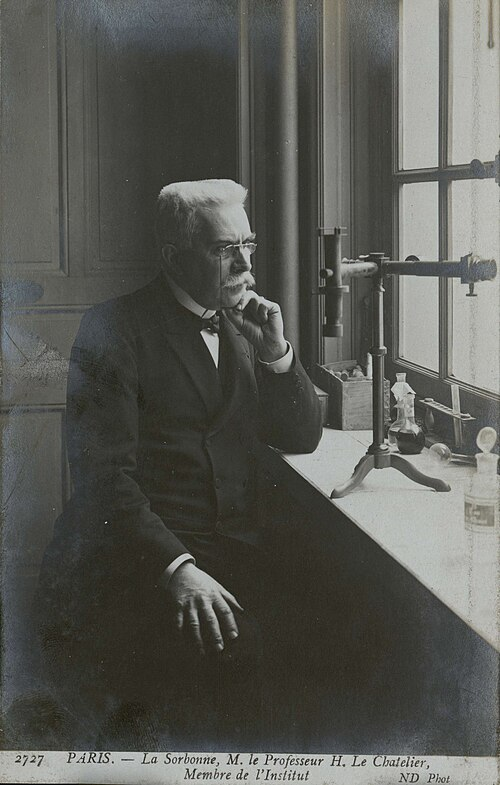
\includegraphics[width=\linewidth]{images/book3/lechatelier.jpg}
\end{minipage}\hfill
\begin{minipage}[t]{0.76\linewidth}\vspace{0pt}
आंरी ले शातेलिए (1850--1936), खनन इंजीनियर और रसायनज्ञ, जिन्होंने
सीमेंट, धातुकर्म और उच्चतापमिति पर काम किया, ने 1884 में अपने नाम से जुड़ा
``\omterm{def:b2:equilibrium-shifts:shift}{साम्य के विस्थापन} का नियम'' कहा। उन्होंने लगभग 1901 में दाब के अंतर्गत तत्वों से
अमोनिया बनाने का प्रयास भी किया था; उनके उपकरण में एक विस्फोट ने
वह प्रयास समाप्त कर दिया। (छायाचित्र: अज्ञात लेखक, CC BY-SA 4.0, विकिमीडिया कॉमन्स।)
\end{minipage}
\end{history}

\section{किसी संश्लेषण का इष्टतमीकरण}

\subsection*{अमोनिया}

\begin{omfigure}
\begin{tikzpicture}
\begin{axis}[
  width=0.78\linewidth, height=6.2cm, xmin=500, xmax=1000, ymin=0, ymax=0.9,
  axis x line=bottom, axis y line=left, xlabel={$T$ (K)},
  ylabel={\ce{NH3} का साम्य मोल अंश},
  tick label style={font=\small}, label style={font=\small}, clip=false]
\addplot[omThm, very thick] table[x=T, y=p300] {figdata/out/bachelor-2-vant-hoff-b.dat};
\addplot[omDef, very thick] table[x=T, y=p200] {figdata/out/bachelor-2-vant-hoff-b.dat};
\addplot[omProp, very thick] table[x=T, y=p50] {figdata/out/bachelor-2-vant-hoff-b.dat};
\addplot[black!60, very thick] table[x=T, y=p1] {figdata/out/bachelor-2-vant-hoff-b.dat};
\node[omThm, font=\scriptsize, anchor=south west] at (axis cs:600,0.70) {\qty{300}{bar}};
\node[omDef, font=\scriptsize, anchor=north east] at (axis cs:612,0.52) {\qty{200}{bar}};
\node[omProp, font=\scriptsize, anchor=north east] at (axis cs:578,0.30) {\qty{50}{bar}};
\node[black!60, font=\scriptsize, anchor=south west] (onebar) at (axis cs:520,0.13) {\qty{1}{bar}};
\draw[black!60] (onebar.south west) -- (axis cs:512,0.075);
\draw[dotted] (axis cs:723,0) -- (axis cs:723,0.253);
\fill[omDef] (axis cs:723,0.253) circle (1.6pt);
\end{axis}
\end{tikzpicture}

{\small नाइट्रोजन और हाइड्रोजन के 1 : 3 मिश्रण (आदर्श गैसें) से अमोनिया का साम्य
मोल अंश, चार दाबों पर ताप के सापेक्ष, सारणीबद्ध गिब्स ऊर्जाओं से
परिकलित। दाब इसे बढ़ाता है, ताप
घटाता है; बिंदु \qty{723}{K} और \qty{200}{bar} को चिह्नित करता है।}
% ledger: janafG:NH3.500, janafG:NH3.600, janafG:NH3.700, janafG:NH3.800, janafG:NH3.900, janafG:NH3.1000 (computed in figdata/bachelor-2/vant-hoff.py)
\end{omfigure}

संश्लेषण \omterm{def:b2:reaction-enthalpy:exothermic}{ऊष्माक्षेपी} है और गैस के चार अणुओं को दो में बदलता है: ऊपर की
प्रतिज्ञप्तियों से, निम्न ताप और उच्च दाब अमोनिया के अनुकूल हैं।
\qty{1}{bar} और कमरे के ताप पर साम्य लगभग पूर्ण है, परंतु
अभिक्रिया चलती ही नहीं: नाइट्रोजन का त्रिक आबंध केवल किसी
उत्प्रेरक पर टूटता है, और लोहे का उत्प्रेरक कई सौ डिग्री पर ही
काम करता है। इसलिए संयंत्र चुनते हैं:
\begin{itemize}
  \item दर के लिए पर्याप्त ऊँचा ताप, उत्प्रेरक जितना नीचा होने दे
        (लगभग \qty{700}{K});
  \item ताप के कारण खोई लब्धि वापस पाने के लिए उच्च दाब, जो
        संपीडन और मोटी दीवार वाले पात्रों की लागत से सीमित है;
  \item एक पाश: परिवर्तक से निकलने वाली गैस ठंडी की जाती है, अमोनिया संघनित होकर
        हटा दी जाती है, और अरूपांतरित गैस ताज़ा फ़ीड के साथ पुनश्चक्रित होती है;
        एक छोटा \omterm{def:b2:equilibrium-shifts:single-pass}{निष्कासन} आर्गन और मेथेन को हटाता है जो अन्यथा
        संचित होती जातीं।
\end{itemize}

\begin{definition}[एकल-पारण रूपांतरण, पुनश्चक्रण, निष्कासन]\label{def:b2:equilibrium-shifts:single-pass}
पुनश्चक्रण वाले प्रक्रम में \emph{एकल-पारण रूपांतरण}\index{एकल-पारण रूपांतरण}
किसी अभिकारक का वह अंश है जो रिएक्टर से एक बार गुज़रने में रूपांतरित
होता है; अरूपांतरित भाग, उत्पाद से अलग करके, रिएक्टर के प्रवेश पर
\emph{पुनश्चक्रण}\index{पुनश्चक्रण} के रूप में लौटाया जाता है;
\emph{निष्कासन}\index{निष्कासन} पुनश्चक्रण से लगातार निकाली जाने वाली एक छोटी धारा है,
जो अक्रिय स्पीशीज़ को संचित होने से रोकती है।
\end{definition}

\begin{omfigure}
\begin{tikzpicture}[font=\small, >={Stealth}, box/.style={draw, thick, rounded corners=2pt, minimum width=2.1cm, minimum height=1.0cm, align=center, fill=white}]
  \node[box] (comp) at (0,0) {संपीडक};
  \node[box] (conv) at (3.6,0) {परिवर्तक\\ (उत्प्रेरक)};
  \node[box] (cond) at (7.2,0) {शीतक और\\ पृथक्कारी};
  \draw[->, thick] (-3.9,0) -- (comp) node[pos=0.0, above right] {ताज़ा \ce{N2 + 3H2}};
  \draw[->, thick] (comp) -- (conv);
  \draw[->, thick] (conv) -- (cond);
  \draw[->, thick, omDef] (cond.south) -- ++(0,-1.0) node[below] {द्रव अमोनिया};
  \draw[->, thick, omThm] (cond.north) -- ++(0,0.9) -| (comp.north);
  \node[omThm, above] at (2.6,1.4) {पुनश्चक्रण (अरूपांतरित गैस)};
  \draw[->, thick, black!60] (6.1,1.4) -- (6.1,2.1) node[above] {निष्कासन};
\end{tikzpicture}

{\small अमोनिया पाश। हर पारण गैस के केवल एक भाग को रूपांतरित करता है; अमोनिया
संघनित करके अलग की जाती है, और शेष को फिर से संपीडित करके ताज़ा
फ़ीड के साथ वापस भेजा जाता है। \omterm{def:b2:equilibrium-shifts:single-pass}{निष्कासन} आर्गन और मेथेन को, जो अभिक्रिया नहीं
करतीं, जमा होने से रोकता है।}
\end{omfigure}

\begin{history}[हाबर और बॉश]
\begin{minipage}[t]{0.15\linewidth}\vspace{0pt}
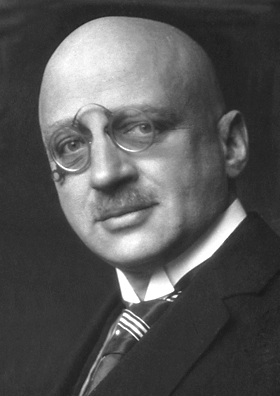
\includegraphics[width=\linewidth]{images/book3/haber.png}
\end{minipage}\hspace{0.01\linewidth}%
\begin{minipage}[t]{0.15\linewidth}\vspace{0pt}
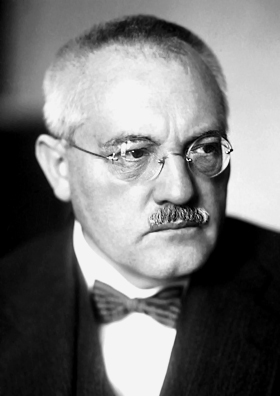
\includegraphics[width=\linewidth]{images/book3/bosch.jpg}
\end{minipage}\hfill
\begin{minipage}[t]{0.66\linewidth}\vspace{0pt}
फ़्रिट्ज़ हाबर (1868--1934) ने दाब के अंतर्गत अमोनिया का साम्य मापा
और, 1909 में, उसे प्रयोगशाला के एक परिवर्तक से ऑस्मियम
उत्प्रेरक के ऊपर लगातार प्रवाहित कराया। कार्ल बॉश (1874--1940) ने इसे उद्योग बनाया,
दाब के अंतर्गत गर्म हाइड्रोजन को सहने वाले इस्पात के पात्रों और सस्ते लोहे के
उत्प्रेरक के साथ; पहला संयंत्र 1913 में चालू हुआ। हाबर को 1918 में और बॉश को
1931 में नोबेल पुरस्कार मिला। (नोबेल फ़ाउंडेशन के चित्र: सार्वजनिक अधिकार-क्षेत्र, विकिमीडिया
कॉमन्स।)
\end{minipage}
\end{history}

\subsection*{सल्फ़र ट्राइऑक्साइड}

संपर्क प्रक्रम में \ce{2SO2(g) + O2(g) <=> 2SO3(g)} (लिखे गए समीकरण के लिए $\Delta_r H^\circ =
\qty{-197.8}{kJ/mol}$) वैनेडियम ऑक्साइड के
उत्प्रेरक पर, जो केवल गर्म होने पर सक्रिय है, कई रुद्धोष्म संस्तरों में चलता है। हर संस्तर में
मुक्त ऊष्मा ताप बढ़ाती है, जो $K^\circ$ घटाता है; जब गैस साम्य वक्र तक
पहुँचती है तो रूपांतरण रुक जाता है। संस्तरों के बीच ठंडा करना उसे
फिर ऐसे ताप पर ले आता है जहाँ साम्य अधिक रूपांतरण की अनुमति देता है।
% ledger: dfh:SO2_g, dfh:SO3_g

\begin{omfigure}
\begin{tikzpicture}
\begin{axis}[
  width=0.72\linewidth, height=6.4cm, xmin=600, xmax=900, ymin=0, ymax=1.08,
  axis x line=bottom, axis y line=left, xlabel={$T$ (K)},
  ylabel={\ce{SO2} का रूपांतरण}, tick label style={font=\small},
  label style={font=\small}, clip=false]
\addplot[black, very thick] table[x=T, y=X] {figdata/out/bachelor-2-vant-hoff-c.dat};
\addplot[omThm, thick] table[x=T, y=X] {figdata/out/bachelor-2-vant-hoff-bed1.dat};
\addplot[omThm, thick] table[x=T, y=X] {figdata/out/bachelor-2-vant-hoff-bed2.dat};
\addplot[omThm, thick] table[x=T, y=X] {figdata/out/bachelor-2-vant-hoff-bed3.dat};
\draw[->, omDef, thick] (axis cs:892.8,0.676) -- (axis cs:712,0.676);
\draw[->, omDef, thick] (axis cs:784.4,0.924) -- (axis cs:712,0.924);
\node[font=\scriptsize, anchor=south west] at (axis cs:860,0.84) {साम्य};
\node[omThm, font=\scriptsize, anchor=west] at (axis cs:800,0.24) {संस्तर 1 (रुद्धोष्म)};
\node[omDef, font=\scriptsize, anchor=south] at (axis cs:800,0.68) {शीतलन};
\end{axis}
\end{tikzpicture}

{\small ताप के सापेक्ष \ce{SO2} का \ce{SO3} में साम्य रूपांतरण
(काला), \qty{1}{bar} पर \qty{10}{\percent} \ce{SO2}, \qty{11}{\percent}
\ce{O2} वाले एक मॉडल फ़ीड के लिए, और तीन रुद्धोष्म संस्तरों से गैस का पथ
(लाल, अभिक्रिया द्वारा गैस को गर्म करने से ताप में बढ़ता हुआ), संस्तरों के बीच
ठंडा किया गया (नीला)।}
% ledger: janafG:SO2.600, janafG:SO2.700, janafG:SO2.800, janafG:SO2.900, janafG:SO3.600, janafG:SO3.700, janafG:SO3.800, janafG:SO3.900 (computed in figdata/bachelor-2/vant-hoff.py; feed and adiabatic rise are model values)
\end{omfigure}

\section{अभ्यास}

\begin{exercise}[$\star$]\label{exo:b2:equilibrium-shifts:1}
\qty{298}{K} पर $K^\circ$ परिकलित कीजिए, उस अभिक्रिया के लिए जिसका $\Delta_r G^\circ =
\qty{-32.8}{kJ/mol}$ है, फिर $\Delta_r G^\circ = \qty{+32.8}{kJ/mol}$ के लिए।
$\Delta_r G^\circ$ का कौन-सा परिवर्तन $K^\circ$ को 100 से गुणा करता है?
\end{exercise}

\begin{exercise}[$\star$]\label{exo:b2:equilibrium-shifts:2}
अमोनिया संश्लेषण के लिए $K^\circ(298) = \num{5.4e5}$ और $\Delta_r H^\circ =
\qty{-91.9}{kJ/mol}$। समाकलित \omterm{thm:b2:equilibrium-shifts:vant-hoff}{वांट हॉफ़ समीकरण} से \qty{400}{K} पर $K^\circ$ का
आकलन कीजिए; सारणियाँ 35.6 देती हैं।
\end{exercise}

\begin{exercise}[$\star$]\label{exo:b2:equilibrium-shifts:3}
इनकी \omterm{def:b2:equilibrium-shifts:variance}{स्वातंत्र्य कोटि} परिकलित कीजिए: (a) अपनी वाष्प के साथ साम्य में द्रव जल;
(b) बंद पात्र में \ce{CaCO3(s) <=> CaO(s) + CO2(g)}; (c) साम्य पर \ce{N2},
\ce{H2}, \ce{NH3}, यादृच्छिक फ़ीड; (d) \ce{C(s) + H2O(g) <=>
CO(g) + H2(g)}।
\end{exercise}

\begin{exercise}[$\star$]\label{exo:b2:equilibrium-shifts:4}
\ce{N2O4(g) <=> 2NO2(g)} के लिए $\Delta_r H^\circ > 0$। नियत दाब पर गर्म करने से,
नियत ताप पर संपीडित करने से, नियत आयतन पर आर्गन मिलाने से साम्य किस दिशा में
विस्थापित होता है?
\end{exercise}

\begin{exercise}[$\star\star$]\label{exo:b2:equilibrium-shifts:5}
\ce{N2(g) + O2(g) <=> 2NO(g)} के लिए $\Delta_r H^\circ = \qty{180.6}{kJ/mol}$,
$\Delta_r S^\circ = \qty{24.8}{J/(K.mol)}$। \qty{298}{K}
और \qty{2000}{K} पर $K^\circ$ (\omterm{def:b2:reaction-free-energy:ellingham-approximation}{एलिंगम सन्निकटन}), और \ce{NO} का मोल अंश परिकलित
कीजिए, जो \qty{2000}{K} पर साम्य में वायु ($x(\ce{N2}) = 0.78$, $x(\ce{O2}) = 0.21$,
थोड़ा उपभुक्त) में होता है। इंजन यह प्रदूषक क्यों बनाते हैं, और ठंडी की गई
निकास गैस में यह बचा क्यों रहता है?
\end{exercise}

\begin{exercise}[$\star\star$]\label{exo:b2:equilibrium-shifts:6}
द्रव प्रावस्था में एक एस्टरीकरण $\mathrm{A + B \rightleftharpoons E + W}$ के लिए
$K^\circ = 4.0$ है (सक्रियताएँ मोल अंश मानी गई हैं)। अम्ल A के
\qty{1.0}{mol} से आरंभ करके, ऐल्कोहॉल B के \qty{1.0}{mol}, फिर
\qty{3.0}{mol} के साथ एस्टर की मात्रा परिकलित कीजिए। $Q$ और $K^\circ$ से समझाइए कि बनते ही
जल को हटाना अभिक्रिया को पूर्णता तक क्यों ले जाता है।
\end{exercise}

\begin{exercise}[$\star\star$]\label{exo:b2:equilibrium-shifts:7}
\qty{298}{K} और \qty{1}{bar} पर \ce{N2O4 <=> 2NO2} के लिए $K^\circ = 0.148$।
\ce{N2O4} के \qty{1}{mol} की वियोजन मात्रा परिकलित कीजिए। फिर
नियत कुल दाब पर \qty{1}{mol} आर्गन मिलाया जाता है: नई
वियोजन मात्रा परिकलित कीजिए, और समझाइए। यदि आर्गन नियत आयतन पर मिलाया जाए
तो क्या होता है?
\end{exercise}

\begin{exercise}[$\star\star$]\label{exo:b2:equilibrium-shifts:8}
अमोनियम क्लोराइड वियोजित होकर ऊर्ध्वपातित होता है, \ce{NH4Cl(s) <=> NH3(g) +
HCl(g)}। \omterm{def:b2:equilibrium-shifts:variance}{स्वातंत्र्य कोटि} परिकलित कीजिए जब गैस केवल ठोस से बनी हो, और जब
कुछ अमोनिया मिलाई गई हो। प्रयोगकर्ता के लिए प्रत्येक स्थिति का क्या अर्थ है?
\end{exercise}

\begin{exercise}[$\star\star$]\label{exo:b2:equilibrium-shifts:9}
सारणियाँ अमोनिया संश्लेषण के लिए \qty{500}{K} पर $K^\circ = 0.0993$ और
\qty{600}{K} पर $K^\circ = \num{1.72e-3}$ देती हैं। उस अंतराल में $\Delta_r H^\circ$
निकालिए और \qty{298}{K} वाले मान से तुलना कीजिए।
\end{exercise}

\begin{exercise}[$\star\star\star$]\label{exo:b2:equilibrium-shifts:10}
\cref{rem:b2:equilibrium-shifts:paradox} का प्रत्युदाहरण सिद्ध कीजिए: अमोनिया संश्लेषण का
$Q$ मात्राओं और कुल दाब से लिखिए, $\partial\ln Q/\partial n(\ce{N2})$ को नियत
$T$ और $p$ पर परिकलित कीजिए, और
$x(\ce{N2})$ पर वह शर्त ज्ञात कीजिए जिसके लिए नाइट्रोजन मिलाना साम्य को
पश्च दिशा में विस्थापित करता है। क्या नियत आयतन पर भी ऐसा हो सकता है?
\end{exercise}

\begin{exercise}[$\star\star\star$]\label{exo:b2:equilibrium-shifts:11}
चूना पत्थर को \qty{10.0}{L} के एक खाली बंद पात्र में
\qty{1100}{K} तक गर्म किया जाता है, जहाँ उसके विघटन के लिए $\Delta_r G^\circ = \qty{1.62}{kJ/mol}$
(\cref{ch:b2:reaction-free-energy})। $K^\circ$ और
कार्बन डाइऑक्साइड का साम्य दाब परिकलित कीजिए। चूना पत्थर के
\qty{0.050}{mol} और \qty{0.200}{mol} के लिए अंतिम अवस्था ज्ञात कीजिए।
\end{exercise}

\begin{exercise}[$\star\star\star$]\label{exo:b2:equilibrium-shifts:12}
संपर्क प्रक्रम वाले चित्र पर हर संस्तर के निकास पर रूपांतरण और ताप पढ़िए।
समझाइए कि एक अकेला रुद्धोष्म संस्तर, चाहे जितना लंबा हो, इस फ़ीड के साथ लगभग
68\,\% रूपांतरण से आगे क्यों नहीं जा सकता, उत्प्रेरक को पूरे समय ठंडा रखने के बजाय
संस्तरों के बीच गैस को ठंडा क्यों किया जाता है, और अंतिम संस्तर के रूपांतरण को
क्या सीमित करता है।
\end{exercise}

\section{समस्या: अमोनिया पाश}

\begin{problem}[{सप्ताहांत समस्या --- अमोनिया संश्लेषण का साम्य स्थिरांक
और उसकी ताप-निर्भरता, परिवर्तक की परिस्थितियों पर संघटन,
दाब, ताप और अक्रिय गैसों से होने वाले विस्थापन, और
पाश}]
\label{pb:b2:equilibrium-shifts:1}
अमोनिया रससमीकरणमितीय फ़ीड से \ce{N2(g) + 3H2(g) <=> 2NH3(g)} द्वारा बनाई जाती है।
आँकड़े: \qty{298.15}{K} पर $\Delta_f H^\circ(\ce{NH3}) = \qty{-45.94}{kJ/mol}$,
$S^\circ_m$ (\unit{J/(K.mol)}) \ce{NH3} 192.77, \ce{N2} 191.61, \ce{H2} 130.68;
सारणियाँ \qty{700}{K} पर $\Delta_f G^\circ(\ce{NH3}) = \qty{+27.19}{kJ/mol}$ और
\qty{800}{K} पर \qty{+38.66}{kJ/mol} देती हैं। गैसें आदर्श हैं;
$R = \qty{8.314}{J/(K.mol)}$।
% ledger: dfh:NH3_g, s0:NH3_g, s0:N2_g, s0:H2_g, janafG:NH3.700, janafG:NH3.800

\medskip
\noindent\textbf{भाग I --- स्थिरांक।}
\begin{enumerate}
  \item \qty{298}{K} पर $\Delta_r H^\circ$, $\Delta_r S^\circ$ और $\Delta_r G^\circ$,
        और $K^\circ(298)$ परिकलित कीजिए।
  \item सारणियों से \qty{700}{K} और \qty{800}{K} पर $K^\circ$ परिकलित कीजिए।
  \item इन दो मानों से \qty{700}{K} और \qty{800}{K} के बीच माध्य $\Delta_r H^\circ$
        निकालिए, और प्रश्न 1 से तुलना कीजिए।
  \item दो सारणीबद्ध मानों से \omterm{thm:b2:equilibrium-shifts:vant-hoff}{वांट हॉफ़ समीकरण} द्वारा $K^\circ(\qty{723}{K})$ का
        आकलन कीजिए।
  \item \qty{298}{K} के आँकड़ों से \omterm{def:b2:reaction-free-energy:ellingham-approximation}{एलिंगम सन्निकटन} में $K^\circ(\qty{723}{K})$
        परिकलित कीजिए, और अंतर पर टिप्पणी कीजिए।
\end{enumerate}

\medskip
\noindent\textbf{भाग II --- परिवर्तक में साम्य।}
\begin{enumerate}[resume]
  \item \qty{1}{mol} \ce{N2} और \qty{3}{mol} \ce{H2} के फ़ीड से, प्रगति $\xi$ पर
        मात्राएँ और कुल मात्रा लिखिए।
  \item दिखाइए कि, $x$ को अमोनिया का मोल अंश मानने पर, \ce{N2} और \ce{H2} के मोल अंश
        $(1-x)/4$ और $3(1-x)/4$ हैं।
  \item दिखाइए कि $\dfrac{x}{(1-x)^2} = \dfrac{\sqrt{27}}{16}\,\dfrac{p}{p^\circ}\,
        \sqrt{K^\circ}$।
  \item \qty{723}{K} और \qty{1}{bar} पर $x$ परिकलित कीजिए।
  \item \qty{723}{K} और \qty{200}{bar} पर $x$ परिकलित कीजिए।
  \item निकाय की \omterm{def:b2:equilibrium-shifts:variance}{स्वातंत्र्य कोटि} परिकलित कीजिए और समझाइए कि $T$ और $p$
        संघटन को क्यों नियत कर देते हैं।
\end{enumerate}

\medskip
\noindent\textbf{भाग III --- विस्थापन।}
\begin{enumerate}[resume]
  \item बिना परिकलन के बताइए, दाब बढ़ने पर साम्य किस दिशा में खिसकता
        है? ताप बढ़ने पर?
  \item नाइट्रोजन बनाने में प्रयुक्त वायु के साथ आर्गन प्रवेश करती है। नियत कुल
        दाब पर उसकी उपस्थिति साम्य को कैसे विस्थापित करती है?
  \item साम्य पर किसी मिश्रण में $x(\ce{N2}) = 0.30$ है। क्या नियत $T$ और $p$ पर थोड़ी
        नाइट्रोजन मिलाना इसे अग्र दिशा में विस्थापित करता है या पश्च?
  \item क्या नियत आयतन पर उत्तर बदल जाएगा?
  \item गैस के परिवर्तक में लौटने से पहले उसकी अमोनिया संघनित करके
        अलग कर दी जाती है। इससे परिवर्तक के प्रवेश पर $Q$ का क्या होता है?
\end{enumerate}

\medskip
\noindent\textbf{भाग IV --- पाश।}
\begin{enumerate}[resume]
  \item गैस परिवर्तक से \qty{18}{\percent} अमोनिया के साथ निकलती है, जो
        साम्य मान से नीचे है। वास्तविक परिवर्तक साम्य तक क्यों नहीं
        पहुँचता?
  \item रससमीकरणमितीय फ़ीड से $x(\ce{NH3}) = 0.18$ के संगत हाइड्रोजन का
        \omterm{def:b2:equilibrium-shifts:single-pass}{एकल-पारण रूपांतरण} परिकलित कीजिए।
  \item अरूपांतरित गैस पुनश्चक्रित होती है। स्थायी संचालन में प्रति इकाई समय
        ताज़ा \ce{N2} का \qty{1.00}{mol} प्रवेश करता है: कितनी अमोनिया निकलती है, और प्रति
        इकाई समय कितनी नाइट्रोजन परिवर्तक से गुज़रती है?
  \item \omterm{def:b2:equilibrium-shifts:single-pass}{पुनश्चक्रण} से थोड़ी गैस का निष्कासन क्यों आवश्यक है?
  \item परिवर्तक को \qty{500}{K} पर क्यों नहीं चलाया जाता, जहाँ साम्य
        कहीं अधिक अनुकूल है?
  \item आदर्श-गैस मॉडल में, रससमीकरणमितीय फ़ीड के लिए \qty{723}{K} और
        \qty{200}{bar} पर अमोनिया का साम्य मोल अंश बताइए।
\end{enumerate}
\end{problem}
